One important application of MultiVariate Normals is to define the class conditional densities in a generative classifier: $p(\bm{x}|y=c,\bm{\theta}) = \mathcal{N}(\bm{x}|
\bm{\mu}_{c}, \bm{\Sigma}_{c})$\\
The resulting technique is called discriminant analysis even though it is a generative
not a discriminant classifier. 
\paragraph{Quadratic discriminant analysis (QDA)}
\begin{align*}
    p(y=c|\bm{x},\bm{\theta}) 
    &= \dfrac{p(y=c|\bm{\theta})p(\bm{x}|y=c,\bm{\theta})}
    {\su{c'}{}p(y=c'|\bm{\theta})p(\bm{x}|y=c',\bm{\theta})}\\
    &=\dfrac{\pi_{c}\lvert 2\pi\bm{\Sigma_{c}}\rvert^{-\frac{1}{2}}exp\left(
    -\frac{1}{2}(\bm{x}-\bm{\mu}_{c})^{T}\bm{\Sigma_{c}}^{-1}(\bm{x}-\bm{\mu}_{c})\right)}
    {\su{c'}{}\pi_{c'}\lvert 2\pi\bm{\Sigma_{c'}}\rvert^{-\frac{1}{2}}exp\left(
    -\frac{1}{2}(\bm{x}-\bm{\mu}_{c'})^{T}\bm{\Sigma_{c'}}^{-1}(\bm{x}-\bm{\mu}_{c'})
\right)}
\end{align*}

\paragraph{Linear discriminant analysis (LDA)}
Let us assume that the covariance matrices are shared across classes, $\bm{\Sigma}_{c=}
\bm{\Sigma}$ then 
\begin{align*}
    \pi_{c}exp\left(-\frac{1}{2}(\bm{x}-\bm{\mu}_{c'})^{T}\bm{\Sigma_{c'}}^{-1}(\bm{x}-
        \bm{\mu}_{c'})\right)\\
    &= \pi_{c}exp\left(-\dfrac{1}{2}\bm{x}^{T}\bm{\Sigma}^{-1}\bm{x}+\dfrac{1}{2}
        \left(\bm{\mu}_{c}^{T}\bm{\Sigma}^{-1}\bm{x}\right)^{T}
        + \dfrac{1}{2}\bm{\mu}_{c}^{T}\bm{\Sigma}^{-1}\bm{x} -\dfrac{1}{2}\bm{\mu}_{c}^{T}
        \bm{\Sigma}^{-1}\bm{\mu}_{c} \right)
        \\
    &= exp\left(\bm{\mu}_{c}^{T}\bm{\Sigma}^{-1}\bm{x} -\dfrac{1}{2}\bm{\mu}_{c}^{T}
        \bm{\Sigma}^{-1}\bm{\mu}_{c} + \log(\pi_{c})\right)exp\left(-
        \dfrac{1}{2}\bm{x}^{T}\bm{\Sigma}^{-1}\bm{x}\right)
\end{align*}

Then
\begin{align*}
    p(y=c|\bm{x},\bm{\theta})
    &=\dfrac{\pi_{c}\lvert 2\pi\bm{\Sigma_{c}}\rvert^{-\frac{1}{2}}exp\left(
            \bm{\mu}_{c}^{T}\bm{\Sigma}^{-1}\bm{x} -\dfrac{1}{2}\bm{\mu}_{c}^{T}
        \bm{\Sigma}^{-1}\bm{\mu}_{c} + \log(\pi_{c})\right)exp\left(
        \dfrac{1}{2}\bm{x}^{T} \bm{\Sigma}^{-1}\bm{x}\right)}
    {\su{c'}{}\pi_{c'}exp\left( \bm{\mu}_{c'}^{T}\bm{\Sigma}^{-1}\bm{x} -\dfrac{1}{2}
        \bm{\mu}_{c'}^{T} \bm{\Sigma}^{-1}\bm{\mu}_{c'} + \log(\pi_{c'})\right)exp\left(
        \dfrac{1}{2}\bm{x}^{T} \bm{\Sigma}^{-1}\bm{x}\right)}\\
    &= \dfrac{e^{\bm{\beta}_{c'}^{T}\bm{x}+\gamma_{c'}}}
    {\su{c'}{}e^{\bm{\beta}_{c}^{T}\bm{x}+\gamma_{c}}}\\
    &= \mathcal{S}(\eta)_{c}
\end{align*}
With 
$ \begin{cases}
    \gamma_{c} = \frac{1}{2}\bm{\mu}_{c}^{T}\bm{\Sigma}^{-1}\mu_{c} + \log(\pi_{c})\\
    \beta_{c} = \bm{\Sigma}^{-1}\bm{\mu}_{c}\\
    \eta^{T} = \left[\beta_{1}^{T}\bm{x}+\lambda_{1}, \ldots, 
    \beta_{c}^{T}\bm{x}+\lambda_{c}\right]\\
    \mathcal{S}\text{ is the \textbf{softmax} function}
\end{cases} $
The softmax function is so-called since it acts a bit like the max function.
Let us divide each $\eta_{c}$ by a constant $T$ called the \textbf{temperature}, 
\begin{center}
    $\displaystyle\lim_{T\to 0}\mathcal{S}\left(\frac{\eta}{T}\right)_{c} = 
    \begin{cases}
        1 \text{ if } c=\displaystyle\argmax_{c'}\eta_{c'}\\
        0 \text{ otherwise}
    \end{cases}$
\end{center}
In other words, at low temperatures, the distribution spends essentially all of its time
in the most probable state, whereas at high temperatures, it visits all states uniformly.
Note that this terminology comes from the area of statistical physics, where it is common
to use the \textbf{Boltzmann distribution}, which has the same form as the softmax
function.\\
This terminology comes from the statistical physics it is common to use the 
\emph{Boltzmann distribution}, which has the same form as the \emph{softmax} function.\\
If we apply the \emph{log} function we end up with a linear function of $\bm{x}$, thus 
\tR{the decision boundary between any two classes, say $c$ and $c'$, will be a straight 
line}.
\begin{align*}
    & p(y=c|\bm{x},\bm{\theta}) = p(y=c'|\bm{x},\bm{\theta}) \\
&\Leftrightarrow \beta_{c}^{T}\bm{x} + \gamma_{c} = \beta_{c'}^{T}\bm{x} + \gamma_{c'}\\
&\Leftrightarrow \bm{x}^{T}(\beta_{c'} + \beta_{c}) = \gamma_{c'} - \gamma_{c}
\end{align*}

\subparagraph{Two-class LDA}
\begin{align*}
    \gamma_{1} - \gamma_{0} 
    &= \dfrac{1}{2}\bm{\mu}_{1}^{T}\Sigma^{-1}\bm{\mu}_{1}+
    \dfrac{1}{2}\bm{\mu}_{0}^{T}\Sigma^{-1}\bm{\mu}_{0} +
    \log\left(\frac{\pi_{1}}{\pi_{0}}\right)\\
    &= \dfrac{1}{2}\left(\bm{\mu}_{1} - \bm{\mu}_{0}\right)^{T}\Sigma^{-1}
    \left(\bm{\mu}_{1} + \bm{\mu}_{0}\right) + \log\left(\frac{\pi_{1}}{\pi_{0}}\right)
\end{align*}
Then in defining 
\begin{center}
    $\begin{cases}
        \bm{w} = \beta_{1} - \beta_{0} = \bm{\Sigma}^{-1}\left(\bm{\mu}{1}-\bm{\mu}{0}
        \right)\\
        \bm{x}_{0} = \dfrac{1}{2}\left(\bm{\mu}_{1} + \bm{\mu}_{0}\right) - 
        \left(\bm{\mu}_{1} - \bm{\mu}_{0}\right)\dfrac{\log\left(\frac{\pi_{1}}{\pi_{0}}
        \right)}{\left(\bm{\mu}_{1} - \bm{\mu}_{0}\right)^{T}\Sigma^{-1}
    \left(\bm{\mu}_{1} - \bm{\mu}_{0}\right)}
    \end{cases}$
\end{center}
Hence we can observe the similarity with logistic regression:
\begin{center}
    \enc{$p(y=1|\bm{x},\bm{\theta}) = sigm\left(\bm{w}^{T}(\bm{x} - \bm{x}_{0})\right)$}
\end{center}
\begin{figure}[H]
    \begin{center}
        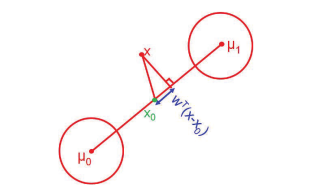
\includegraphics[width=.5\textwidth]{./chaps/32_sec/images/2_geometry_lda.png}
    \end{center}
    \caption{Geometry of LDA in the 2 class case where $\bm{\Sigma}_{1} = \bm{\Sigma}_{0}
= \bm{I}$}
    \label{fig:2_geometry_lda}
\end{figure}

\subparagraph{MLE for discriminant analysis}
The \emph{log-likelihood} function is as follows:
\begin{center}
    $\log\left(p(\mathcal{D}|\theta)\right) = 
    \su{i=1}{N}\su{c=1}{C}\mathbb{1}(y_{i}=c)\log(\pi_{c}) + \su{c=1}{C}\left[
        \su{i:y_{i}=c}{}\log\left(\mathcal{N}(\bm{x}|\bm{\mu}_{c},\bm{\Sigma}_{c})\right)
\right]$
\end{center}

\subparagraph{Strategies for preventing the overfitting}
Even if \textit{speed} and \textit{simplicity} are the attractive aspects of MLE, it can
badly overfit in high dimensions.\\
In particular the MLE for a full covariance matrix is singular if $N_{c} < D$, and even
when $N_{c} > D$ the MLE can be ill-conditioned, meaning close to singular.\\
Some solution to this problem:
\begin{itemize}
    \item use a diagonal covariance matrix for each class, this assumes the features are
        conditionally independent, this is equivalent to using a naive Bayes classifier.
    \item use the full covariance matrix but force it to be the same for all classes, 
        $\Sigma_{c} = \Sigma$, this is equivalent to \textit{parameter sharing} and is
        equivalent to LDA.
    \item Use a diagonal matrix and force it to be shared.
    \item use a diagonal covariance, but impose a prior and then integrate it out. If we 
        use a conjugate prior this is analogous to the Bayesian naive Bayes.
    \item fit a full or a diagonal covariance matrix by MAP estimation.
    \item Project the data into a low dimensional subspace and fit the Gaussian there.
\end{itemize}

\subparagraph{Regularized LDA*}
Assume we tie the covariance matrices, so $\bm{\Sigma_{c}} = \bm{\Sigma}$ as in LDA and 
furthermore we perform MAP estimation of $\bm{\Sigma}$ using an inverse Wishart prior 
of the form $IW(diag(\hat{\bm{\Sigma}}_{mle}), \nu_{0})$
\begin{center}
$\hat{\bm{\Sigma}} = \lambda diag(\hat{\bm{\Sigma}}_{mle}) =
(1-\lambda)\hat{\bm{\Sigma}}_{mle}$
\end{center}
where $\lambda$ controls the amount of regularization which is related to the strength of the prior $\nu_{0}$

\subparagraph{Nearest shruken centroids classifier}
A disadvantage of \textit{diagonal LDA} is it depends on all of the features.\\
An idea can be to perform MAP estimation for the diagonal LDA with a sparsity-promoting 
(Laplace).\\
More precisely define
\begin{itemize}
    \item $\mu_{cj}$ class-specific feature mean 
    \item $m_{j}$ class-independent feature mean
    \item $\Delta_{cj}$ class-specific offset
\end{itemize}
Then $\mu_{cj} = m_{j} + \Delta_{cj}$
In putting a prior on the $\Delta_{cj}$ terms to encourage them to be strictly zero and 
compute a MAP estimate. If, for feature $j$ we find that $\Delta_{cj}=0$ for all $c$, 
then feature $j$ will play no role in teh classification decision. Thus features that are 
not discriminative are automatically ignored.

\paragraph{Inference in jointly Gaussian distribution}
Suppose $\bm{x} = (x_{1}, x_{2})$, then\\
$\bm{\mu} = \begin{pmatrix}
    \mu_{1}\\
    \mu_{2}
\end{pmatrix},
\bm{\Sigma} = \begin{pmatrix}
    \Sigma_{11} & \Sigma_{12}\\
    \Sigma_{21} & \Sigma_{22}
\end{pmatrix},
\bm{\Lambda} = \bm{\Sigma}^{-1} = \begin{pmatrix}
    \Lambda_{11} & \Lambda_{12}\\
    \Lambda_{21} & \Lambda_{22}
\end{pmatrix} $\\
Thus the marginals are given by: 
$\begin{cases}
    p(x_{1}) = \mathcal{N}(x_{1}|\mu_{1}, \Sigma_{11})\\
    p(x_{2}) = \mathcal{N}(x_{2}|\mu_{2}, \Sigma_{22})
\end{cases}$\\
and the posterior conditional is given by: 
\tR{
\begin{align*}
    p(x_{1}|x_{2}) &= \mathcal{N}(x_{1}|\mu_{1|2},\Sigma_{1|2})\\
    \mu_{1|2} &= \mu_{1} + \Sigma_{12}\Sigma_{22}^{-1}(x_{2} -\mu_{2})\\
              &= \mu_{1} - \Lambda_{11}^{-1}\Lambda_{12}(x_{2} -\mu_{2})\\
              &= \Sigma_{1|2} \left(\Lambda_{11}\mu_{1} - \Lambda_{12}(x_{2}-\mu_{2})
              \right)\\
    \Sigma_{1|2} &= \Sigma_{11} - \Sigma_{12}\Sigma_{22}^{-1}\Sigma_{21}\\
                 &= \Lambda_{11}^{-1}
\end{align*}
}
The conditional mean is just a linear function of $x_{2}$ and the conditional covariance 
is just a constant matrix that is independent of $x_{2}$






